\section{Risikoabsch�tzung}

\subsection{Risiko - Eintrittswahrscheinlichkeit - Schadenpotenzial}

\begin{itemize}
\item Komplexit�t: Die Schnittstelle zu Lotus Notes kann schwierig zu realisieren sein.
\item Termin: Das Projekt wird nicht zum vereinbarten Termin abgeschlossen.
\item Qualit�t: Die vereinbarten Anforderungen werden nicht erf�llt.
\item Budget: Das Projekt wird teurer als geplant.
\item �nderungen: Die Anforderungen werden nachtr�glich ge�ndert.
\end{itemize}

\begin{table}[h]
\caption{Risiko - Eintrittswahrscheinlichkeit - Schadenpotenzial}
\begin{tabular}[h]{|p{3cm}|p{7cm}|p{4cm}|}
\hline
\textsc{Risiko} & \textsc{Eintrittswahrscheinlichkeit} & \textsc{Schadenpotenzial}\\
\hline
Komplexit�t & 0,5 & 0,5\\
\hline
Termin & 0,25 & 0,25\\
\hline
Qualit�t & 0,2 & 0,35\\
\hline
Budget & 0,05 & 0,5\\
\hline
�nderungen & 0,1 & 0,1\\
\hline
\end{tabular}
\end{table}

\subsection{Risikomatrix}
Die Risikomatrix ist in Abbildung 1 dargestellt.
\begin{figure}[h]
\begin{center}
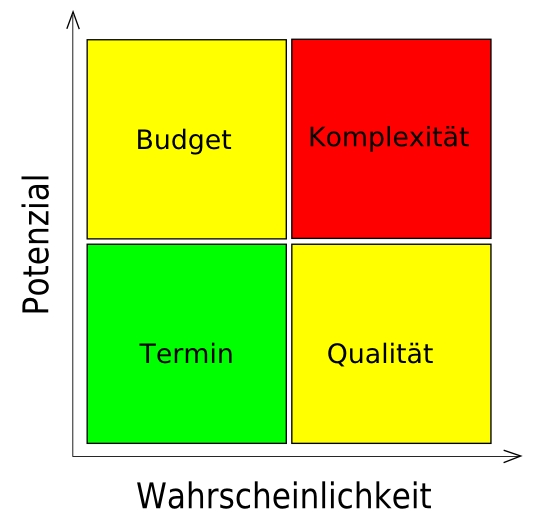
\includegraphics[width=0.8\textwidth]{abbildungen/Wahrscheinlichkeit-Potenzial.jpg}
\caption{Risikomatrix}
\end{center}
\end{figure}

\subsection{Vorbeugema�nahmen}
\begin{itemize}
\item Die Lotus Notes Schnittstelle wird von einem Programmierer implementiert der Erfahrung von dem benutzten Lotus Notes Bibliotheksmodul hat und in der vorgegeben Zeit und mit dem veranschlagtem Budget die Aufgabe erledigen kann.
\item Alternativen f�r M�bel und Hardware bereitstellen um den Zeitplan und das Budget zu halten.
\item St�ndige Terminkontrolle w�hrend des laufenden Projekt um notfalls Studenten oder externe Arbeiter zus�tzlich zu besch�ftigen, aber dadurch werden die Kosten wahrscheinlich steigen.
\item �nderungen der Aufgabenstellung vertraglich ausschlie�en oder eine jeweilige Kostenerh�hung vertraglich festlegen.
\item Um im Kostenbudget zu bleiben kann man den Aufwand und die Kosten mit �hnlichen, schon abgeschlossenen, Projekten vergleichen.
\item Nach jedem erfolgreich erledigten Meilensteine die Ergebnisse vom Auftraggeber absegnen lassen.
\end{itemize}

\subsection{Korrekturma�nahmen}
\begin{itemize}
\item Bei Eintritt des Risikos "Komplexit�t" in Absprache mit dem Auftraggeber Funktionalit�t weglassen oder mehr Zeit investieren oder mehr Leute besch�ftigen, was die Kosten erh�hen wird.
\item Bei Nichtlieferbarkeit von M�beln oder Hardware auf Alternativen zur�ckgreifen.
\item Bei nachtr�glicher �nderung der Aufgabenstellung vertraglich vereinbarte Kostenerh�hung geltend machen und gleichzeitig mehr Zeit veranschlagen.
\end{itemize}